Con este proyecto se propone el desarrollo de un software que ayude a predecir la demanda de productos en diferentes dominios y contetos de gestion de inventarios. Este sistema se realizara tras analizar datos como historial de consumo, esto para poder estimar exactamente las cantidades necesarias de cada producto en periodos mensuales.

La solucion implementara modelos de prediccion de demanda que procesaran la informacion historica para identificar patrones y en base a ellos, generar estimaciones futuras. A partir de estas predicciones, el sistema podra proporcionar informacion relevante para la toma de decisiones, tales como cantidades recomendadas de compra, puntos de reposicion y posibles alertas de desabastecimiento.

Se utilizaran datos reales del año 2021 del sector salud como caso de estudio, que seran complementados con datasets con datos publicos de diferentes dominios esto para poder evaluar el comportamiento del sistema en diferentes contextos.

Adicionalmente, el sistema tendra en cuenta variables como tiempo de entrega de proovedores (lead time) y cantidad de productos disponivle, con el proposito de lograr que el sistema sea lo mas preciso posible.

Esta informacion sera presentada en una interaz que permitira visualizar los resultados de manera comprensible, esto para facilitar su uso por parte del personal encargado de la gestion de inventarios.
\begin{figure}[H]
    \centering
    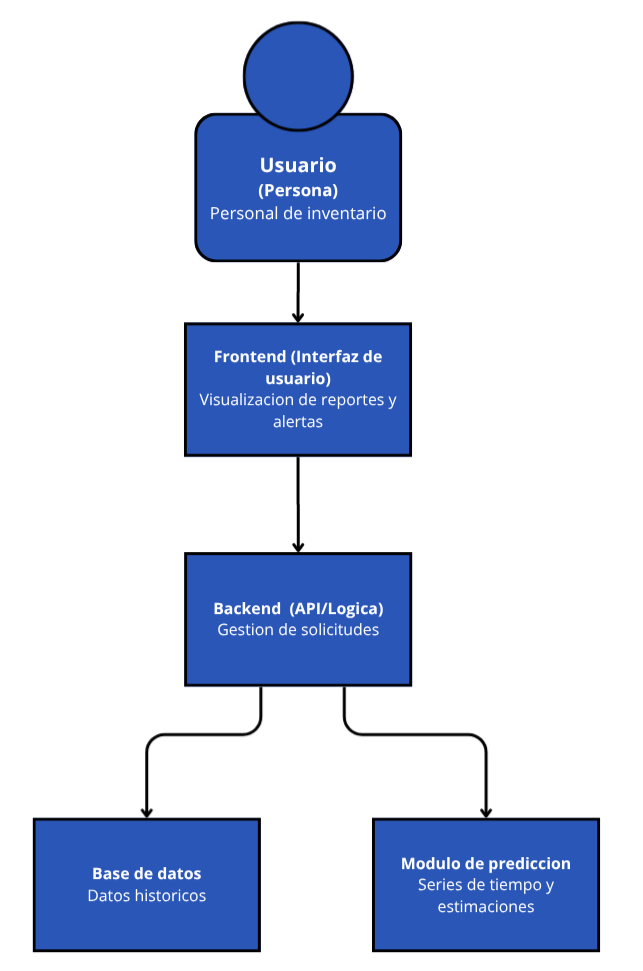
\includegraphics[width=0.5\textwidth]{templatefigures/propuesta.png}
    \caption{Esquema detallado de la propuesta de solucion.}
\end{figure}